\chapter{Introduction}\label{chap:introduction}
This paper is written for the master course \textit{Concepts of Programming Languages} of the department of computer science in the Winter Term 23/24 at the Technical University of Applied Sciences Rosenheim.
    \section{Background}\label{sec:background}
As of the TIOBE Index data as of November 2023, it is reported that there are currently over 150 programming languages in existence. This implies that, up until the present moment, the programming landscape continues to encompass a diverse array of languages, reflecting the dynamic and ever-evolving nature of the field.\cite{tiobeindex} The task of a software engineer at a certain point in the production of software is to select one of these programming languages that is suitable for a particular problem. This can be a science in itself. This very topic has been discussed for around 50 years.\cite{Tharp1982}
The reason for that is that every language has its own paradigms and concepts. One can come up with a solution, selecting a language which fits a lot of problems but not a single one perfect. Or he selects one which fits perfect for a single problem but it is not possible to solve all the other problems.
So the goal would be to select the \textit{right} programming language which suits the requirements and the surrounding of a given problem accordingly.
This spot should be covered by this paper with the comparison of Go and F\# in the context of \ac{fp}.

    \section{Purpose of the Project}\label{sec:purpose}
    The object of this project is to analyze and compare the similarities and differences between two functional programming languages. The selected languages for this comparative study are Go\footnote{Website: \url{https://go.dev} (Accessed on 12/02/2023)} and F\#\footnote{Website: \url{https://dotnet.microsoft.com/languages/fsharp} (Accessed on 12/02/2023)}. Go was chosen as the initial language due to its consistent usage throughout the course, making it mandatory inclusion in the project. 
    In addition to Go, a second programming language is essential for the comparative analysis, and F\# has been selected for this purpose. The inclusion of F\# in this study was a deliberate choice, as explained in section 
    ef{sec:whyfsharp}. By juxtaposing Go and F\#, the project aims to unravel the nuances and divergences in their approaches to \ac{fp} paradigms, shedding light on their distinctive features, strengths, and potential use cases. Through this comparative exploration, the project seeks to contribute valuable insights into the \ac{fp} landscape, providing a nuanced understanding of the strengths and trade-offs associated with these two languages.

    \section{Why F\#?}\label{sec:whyfsharp}
    One of the key reasons for choosing F\# is its status as a functional-first programming language. In contrast to Go's multi-paradigm approach, F\#'s commitment to functional principles provides an excellent opportunity to explore the benefits of implementing code from a pure perspective.
    For a more in-depth understanding of F\#, including its syntax, features, and \ac{fp} principles, readers are encouraged to refer to section \ref{sec:fsharp-overview} and chapter \ref{chap:comparison}.

    \section{Roadmap}\label{sec:roadmap}
    Embedded within this exploration about \ac{fp} is a brief discussion of the \textit{NerdDeck} Flash Card \ac{app} in chapter 2, our practical context for understanding \ac{fp} in action. Besides of that this paper navigates a concise roadmap to compare \ac{fp} in Go and F\#, anchored by an initial overview of \ac{fp} principles in chapter 3. It then swiftly transitions to individual language analyses in chapter 4, spotlighting key design philosophies and features of Go and F\#. The centerpiece is chapter 5, a focused exploration of two critical functional concepts: Algebraic Data Types and First-class Functions. Leveraging code examples, this section illuminates nuances in implementation, providing a succinct yet insightful comparative analysis. The paper concludes in chapter 6, summarizing challenges and outlook from both the project and the comparison. This streamlined roadmap ensures a comprehensive yet condensed examination of \ac{fp} in Go and F\#.

\chapter{Project Overview}\label{chap:project-overview}
    \section{Description of the \textit{NerdDeck} Flash Card Application}\label{sec:description}
    This coding project should illustrate and highlight similarities and differences about \ac{fp} in Go versus F\#.
    \textit{NerdDeck} is app which can help remembering things with flashcards. There exists already such a product called Anki\footnote{Website: \url{https://apps.ankiweb.net} (Accessed on 12/03/2023)} for the same use case. Most parts of Anki are written in Rust and Python.\footnote{Website: \url{https://github.com/ankitects/anki} (Accessed on 12/03/2023)} The difference in \textit{NerdDeck} is that it is written twice, each time in a different programming language, Go and F\#, and the \ac{fp} paradigm should be used. In F\# there will be no problem as it will turn out in section \ref{sec:fsharp-overview} because it is possible to write functional-first code. But as Go is a impure language, the goal is to write it as functional as possible. In addition to that, \textit{NerdDeck} should just use the \ac{cli} as a \ac{gui} while Anki has a own one.

    \section{Requirements}
     The \ac{app} should allow a single user to use the \ac{sm2} alorithm which is used for spaced repetition.\cite{sm2} One of Anki's algroithms is also based on \ac{sm2}.\footnote{Website: \url{https://faqs.ankiweb.net/what-spaced-repetition-algorithm.html} (Accessed on 12/03/2023)} Because \textit{NerdDeck} is build by a student, the requirements are also written from a students perspective. The requirements are written down in table \ref{tab:requirements}. These should not differ too big from other users using this application. The goal is to implement this twice, one time in Go and then in F\#, both in a functional style. The program should act as a \ac{mvp}, so it's possible to do the comparison about \ac{fp}. Because of that and to reduce the complexity, only one deck exists where a user can add new flashcards. They can not be deleted.
    \begin{table}[h]
        \centering
        \begin{tabular}{|m{0.5in}|m{4in}|}
            \hline
            \textbf{ID} & \textbf{Requirement} \\
            \hline
            1 & As a student, I want to create a flashcard inside a deck. \\
            \hline
            2 & As a student, I want to view my flashcards. \\
            \hline
            3 & As a student, I want to know how to use the program. \\
            \hline
            4 & As a student, I want that a flashcard is unique with its question and answer. So no duplicates.  \\
            \hline
            5 & As a student, I want to apply a spaced repetition algorithm to learn with the flashcards. \\
            \hline
        \end{tabular}
        \caption{\textit{NerdDeck} Requirements}\label{tab:requirements}
    \end{table}

    \section{Data}
    For the purpose of this project, a single \ac{json} file is used as a simple and lightweight database to store flashcards. For example in the \ac{json} object in listing \ref{l:flashcardjson}. While this approach is suitable for educational and illustrative purposes, it may not be suitable for production usage due to limitations in scalability and concurrent access. In a production environment, a more robust database solution should be considered, such as a relational database (e.g., PostgreSQL\footnote{Website: \url{https://www.postgresql.org} (Accessed on 12/02/2023)}, MySQL\footnote{Website: \url{https://www.mysql.com} (Accessed on 12/02/2023)}) or a NoSQL database (e.g., MongoDB\footnote{Website: \url{https://www.mongodb.com} (Accessed on 12/02/2023)}). The choice of the database will depend on the specific requirements of the \ac{app}.

    \subsection{Model}
    To be able to fulfill the requirements of table \ref{tab:requirements} a model is needed for a flashcard. These are shown in figure \ref{fig:model}. It is important that allow a user to create multiple flashcards and validate that there is no flashcard with a duplicate question and answer. The ID is generated from the question and answer of the flashcard. This ID acts like a primary key for the model. This model should be used within both languages.

    \begin{figure}
        \centering
        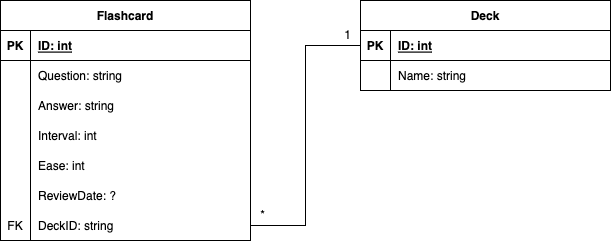
\includegraphics[width=0.4\textwidth]{NerddeckModel.png}
        \caption{Entity-Relationship Model of Flashcard and Deck}\label{fig:model}
    \end{figure}

    \begin{lstlisting}[language=json,firstnumber=1,float=tp, caption={Example of how a flashcard is saved inside a \ac{json} file}, label=l:flashcardjson]
    [{
        "ID": "37268335dd6931045bdcdf926",
        "Question": "What algebraic data types does F# use?",
        "Answer": "Record types and discriminated unions",
        "Repetitions": 1,
        "EasinessFactor": 1.3,
        "NextReview": "2023-12-18T18:17:22.438077+01:00"
    }]   
    \end{lstlisting}

    \section{Functionality Overview and User Interface}
    In figure \ref{fig:screenshotcli} the result of the F\# implementation can be seen, the welcome screen and menu looks the same way in the go implementation.. A user who executes the program can select between 5 choices:        
    \begin{itemize}
        \item \textbf{0. Instructions:} Shows how the program should be used.
        \item \textbf{1. Add Flash Card} Add a Flash Card and saves it into the \ac{json} file.
        \item \textbf{2. View Flash Cards:} Just prints all flashcards from the \ac{json} file on the \ac{cli}.
        \item \textbf{3. Start Learning:} Loads all Flash Cards from the \ac{json} file. Checks all due Flash Cards based on the next review. Learn every Flash Card and then rate each one from 1 to 4 while 1 is bad and 4 is good. Apply the value as input for the \ac{sm2} algorithm and save the result in the \ac{json} file.
        \item \textbf{4. Exit:} Exit the program.
    \end{itemize}

    \begin{figure}
        \centering
        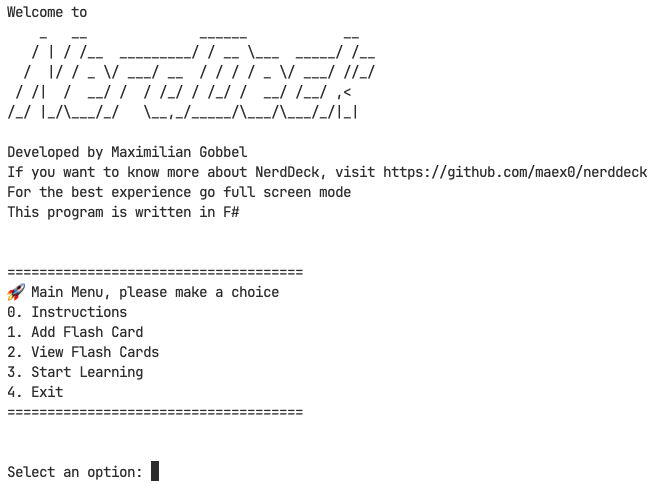
\includegraphics[width=0.8\textwidth]{ScreenshotNerdDeck.png}
        \caption{Screenshot of the \ac{cli}. Shows start of \textit{NerdDeck}.}
        \label{fig:screenshotcli}
    \end{figure}


    \chapter{Overview of functional programming}\label{chap:functional-programming}
    \begin{shaded}
        \noindent
        \glqq{}As software becomes more and more complex, it is more and more important to structure it well. Well-structured software is easy to write, easy to debug, and provides a collection of modules that can be re-used to reduce future programming costs. Conventional languages place conceptual limits on the way problems can be modularized. Functional languages push those limits back.\grqq{} \cite{Hughes1989}
    \end{shaded}
    This should be the motivation considering the usage of \ac{fp}.
    Within the paradigm of \ac{fp}, developers engage with principles that underscore the pursuit of expressive and concise solutions. Rooted in mathematical concepts like lambda calculus, \ac{fp} emerges as a methodology characterized by rigor and elegance.
    
    Key principles integral to \ac{fp} include:
    
    \begin{itemize}
        \item \textbf{Purity:} Strict avoidance of side effects to ensure deterministic behavior.
        \item \textbf{Higher-order functions:} Utilization of functions as parameters and return values for enhanced modularity.
        \item \textbf{Lazy evaluation:} Selective computation, evaluating values only when necessary for optimization.
        \item \textbf{Algebraic data types:} Incorporation of sum- and product-types, as discussed in more detail in Section \ref{sec:algebraic-data-types}.
        \item \textbf{First-class Functions:} A powerful technique, elaborated further in Section \ref{sec:first-class-functions}.
    \end{itemize}
    
    Originating in 1950 with the introduction of the impure language LISP, \ac{fp} has evolved across languages like F\# and Go. F\# strictly adheres to a functional-first approach, emphasizing immutability and mathematical principles, while Go incorporates impure functional elements, showcasing the adaptability of \ac{fp} principles. Additional insights into this topic are expounded upon in Chapter \ref{chap:language-comparison}.
    
    As developers navigate through contrasting algorithms, exploring the interplay between imperative and declarative styles, they reflect on the historical evolution and diversity of \ac{fp} languages. This exploration serves as a testament to the flexibility of programming paradigms and prompts consideration of the nuanced trade-offs between explicit instruction and expressive abstraction within the dynamic context of \ac{fp}.
    
    In conclusion, \ac{fp} equips professionals with a robust set of tools, emphasizing immutability, higher-order functions, and mathematical principles. It not only addresses contemporary challenges in software development but also fosters a deeper understanding of the intricacies involved in designing robust, modular, and expressive code.
    

\section*{Imperative vs. Declarative}

Within the broader spectrum of programming paradigms, the imperative and declarative styles represent two contrasting approaches to articulating code. In the following the two approaches will be shown on a simple algorithm: summing up a array of numbers.

\subsubsection{Imperative Approach}

Algorithm \ref{alg:imperative_sum} exemplifies the imperative paradigm, which guides the computer through computations using explicit steps. Each line of pseudocode provides instructions to the computer on how to perform the calculation, adhering to traditional imperative paradigms.

\begin{algorithm}
    \SetKwInOut{Input}{Input}
    \SetKwInOut{Output}{Output}

    \underline{function SumArray} $(a)$\;
    \Input{Integer Array $a$}
    \Output{Sum of elements in $a$}
    
    \BlankLine
    $result \leftarrow 0$
    
    \ForEach{$element$ \textbf{in} $a$}
    {
        $result \leftarrow result + element$
    }
    
    \Return $result$
    
    \caption{Imperative way of summing up an integer array}
    \label{alg:imperative_sum}
\end{algorithm}

\subsubsection{Declarative Approach}

In contrast, the declarative style, showcased by Algorithm \ref{alg:declarative_sum}, shifts the emphasis from detailing step-by-step procedures to expressing the desired outcome directly. This approach, a hallmark of \ac{fp}, leverages the power of functions and abstraction.

\begin{algorithm}
    \SetKwInOut{Input}{Input}
    \SetKwInOut{Output}{Output}

    \underline{function SumArray} $(a)$\;
    \Input{Integer Array $a$}
    \Output{Sum of elements in $a$}
    
    \BlankLine
    \Return $\sum_{\text{element in } a} \text{element}$
    
    \caption{Declarative way of summing up an integer array}
    \label{alg:declarative_sum}
\end{algorithm}

The juxtaposition of these algorithms not only highlights the difference in coding philosophy but also serves as a tangible exploration of the imperative and declarative styles within the context of \ac{fp}.


\chapter{Introduction to Go and F\#}\label{chap:language-comparison}
In this chapter, we explore the distinctive features of Go and F\#, offering a brief overview of each language.

    \section{Overview of Go}\label{sec:go-overview}
    Go, commonly known as Golang, is employed to build simple, secure, and scalable systems. It is a statically-typed, compiled programming langauge designed by Google engineers Robert Griesemer, Rob Pike, and Ken Thompson in 2007. It is used very widely within big companies like Google, Paypal or Netflix. As an open source language, Go is characterized by: 
    \begin{itemize}
        \item \textbf{Concurrent programming:}  Native support through goroutines and channels for scalable and parallelized applications.
        \item \textbf{Efficiency:} Statically-typed, compiled that produces standalone binaries. Good for deployment in various environments.
        \item \textbf{Flexibility:} Can be used for Cloud \& Network Services, \ac{cli}s, Web Development and Development Operations \& Site Reliability Engineering.
    \end{itemize}
    \cite{GoWebsite}

    \section{Overview of F\#}\label{sec:fsharp-overview}
    F\# is a functional-first programming language developed by Microsoft Research in 2005.
    Besides C\# and Visual Basic, F\# is another programming language within the .NET ecosystem. On the official website of microsoft it is declared as an open-source language that makes it easy to write succinct, robust, and performant code. Microsoft names itself as a leading contributor. F\# has an active community and support \cite{fsharpfoundation}.
    While developing, F\# has a very powerful build-in future called \ac{repl}. Besides of that the key features are:
    \begin{itemize}
        \item \textbf{Functional-first:} Immutable by default, First-class functions, Pattern Matching, Algebraic Data Types 
        \item \textbf{Lightweight syntax:} Type inference and automatic generalization
        \item \textbf{Interoperability:} Access .NET Libraries and APIs (e.g. ASP.NET or Entity Framework). 
    \end{itemize}
    \cite{dotnet}
    \cite{keyfeaturesfsharp}
    Both of the languages are not completely pure.


\chapter{Comparison of functional concepts}\label{chap:comparison}
In order to compare the two languages, the following two functional concepts are examined in more detail: Algebraic Data Types and First-class Functions. 

    \section{Algebraic Data Types}\label{sec:algebraic-data-types}

    Algebraic data types (ADTs) are a cornerstone of functional programming, providing a way to model complex data structures. In Go, ADTs are not directly supported as in languages like F\#, which has native support for discriminated unions and pattern matching. In both F\# and Go, the \texttt{FlashCard} type is used to represent a flashcard, capturing essential information such as the card's ID, question, answer, repetition count, easiness factor, and the next review date. Despite serving the same purpose, there are syntactic and structural differences between the implementations in F\# and Go.

        \subsection*{F\#}
        F\# provides native support for algebraic data types through discriminated unions. Developers can define a set of related values using a discriminated union, and pattern matching allows for concise and expressive handling of these types. This feature enhances the readability and maintainability of F\# code, making it a powerful tool for developers embracing functional programming.


        In listing \ref{l:flashcardfsharp} the \texttt{FlashCard} type is defined using a record type, a lightweight and immutable data structure. The \texttt{FlashCard} record includes fields for \texttt{ID}, \texttt{Question}, \texttt{Answer}, \texttt{Repetitions}, \texttt{EFactor}, and \texttt{NextReview}. Records in F\# automatically provide immutability, making them well-suited for representing data with fixed attributes.


        \subsection*{Go}
        In Go, developers commonly use struct types to represent data structures. While structs provide a way to encapsulate related data, they lack the succinct expressiveness of algebraic data types. Go's approach often involves using interfaces and composition to achieve similar outcomes, but this can lead to more verbose code compared to the concise syntax offered by ADTs.

        The \texttt{FlashCard} type is defined using a struct. Go structs are mutable, and fields can be updated after the struct's creation. The \texttt{FlashCard} struct includes fields for \texttt{ID}, \texttt{Question}, \texttt{Answer}, \texttt{Repetitions}, \texttt{EFactor}, and \texttt{NextReview}. Go uses explicit types for each field, providing a statically typed approach.

\begin{figure}[ht]
    \begin{subfigure}{0.48\textwidth}
        \begin{lstlisting}[language=go, firstnumber=1, caption={FlashCard representation in Go}, label=l:flashcardgo]
    type FlashCard struct {
        ID          string
        Question    string
        Answer      string
        Repetitions int
        EFactor     float64
        NextReview  time.Time
    }
        \end{lstlisting}
    \end{subfigure}\hfill
    \begin{subfigure}{0.48\textwidth}
        \begin{lstlisting}[language=FSharp, firstnumber=1, caption={FlashCard representation in F\#}, label=l:flashcardfsharp]
    type FlashCard =
        { ID : string
        Question : string
        Answer : string
        Repetitions : int
        EFactor : float
        NextReview : DateTime }
        \end{lstlisting}
    \end{subfigure}
    \caption{Comparison of FlashCard representations in Go and F\#}
    \label{fig:flashcardcomparison}
    \end{figure}

    \section{First-class Functions}\label{sec:first-class-functions}
    Both Go and F\# support first-class functions, treating functions as first-class citizens. In Go, functions can be assigned to variables, passed as arguments, and returned as values. The use of anonymous functions, known as closures, is common in Go, enhancing the functional programming paradigm. Similarly, F\# provides robust support for first-class functions, aligning with its functional programming paradigm. Functions in F\# can be assigned to variables, passed as arguments, and returned as values. The language encourages the use of higher-order functions, enabling powerful abstractions through functions.

    \subsection*{F\#}
        \begin{lstlisting}[language=fsharp, firstnumber=1,float=tp, caption={First-class function reresentation in F\#}, label=l:flashcardfunction]
let isDueForReview card =
    card.Repetitions > 0 && card.NextReview <= DateTime.Now
        
let dueFlashcards = List.filter isDueForReview flashcards
        \end{lstlisting}
        
        In this F\# example, we define a first-class function `isDueForReview` that checks if a flashcard is due for review based on specific criteria. We then use this function to filter a list of flashcards.
        
    \subsection*{Go}    
        \begin{lstlisting}[language=go, firstnumber=1, caption={FlashCard representation in F\#}, label=l:flashcardfsharp]
            func isDueForReview(card FlashCard) bool {
                return card.Repetitions > 0 
                && card.NextReview.Before(time.Now())
            }
            
            func filterDueFlashcards(cards []FlashCard) []FlashCard {
                var dueFlashcards []FlashCard
                for _, card := range cards {
                    if isDueForReview(card) {
                        dueFlashcards = append(dueFlashcards, card)
                    }
                }
                return dueFlashcards
            }
            
    
            dueFlashcards := filterDueFlashcards(cards)
            \end{lstlisting}
            
            In this Go example, we define a first-class function `isDueForReview` that checks if a flashcard is due for review based on specific criteria. We then use this function to filter a slice of flashcards and print the result.

    \section{Key Takeaway}\label{sec:keytakeaway}
    In conclusion, when it comes to algebraic data types—a fundamental feature in functional programming—F\# excels with its native support for discriminated unions and pattern matching. While Go developers can achieve similar outcomes using struct types and interfaces, F\# provides a more elegant and concise solution. Both languages support first-class functions, making them suitable choices for developers with different preferences in balancing imperative and functional programming styles.


\chapter{Conclusion}\label{chap:conclusion}
In the exploration of functional programming paradigms within the context of Go and F\#, this paper aimed to analyze and compare key concepts such as Algebraic Data Types and First-class Functions. The \textit{NerdDeck} Flash Card application served as a practical example to illustrate the application of functional programming principles in both languages. The comparison revealed distinctions in their approaches, showcasing F\#'s native support for functional programming and Go's adaptation within its multi-paradigm framework.
    \section{Challenges}\label{sec:challenges}
    The foundation of a good comparison in the context of this paper is to write code as pure as possible to fulfill the paradigm of functional programming. However, challenges arose due to the inherent impurity in both Go and F\#. While F\# aligns more closely with functional programming principles, Go's multi-paradigm nature necessitated creative workarounds to achieve a functional style. This underscored the importance of navigating the balance between functional and imperative programming in each language. The challenges also highlighted the need for a nuanced approach when selecting a language for projects where functional programming principles are a priority.        

    \section{Outlook}\label{sec:outlook}
    Looking ahead, there is potential for further exploration into writing more pure functional code within the \textit{NerdDeck} or similar projects. For this, a pure programming language like for example Haskell\footnote{Website: \url{https://www.haskell.org} (Accessed on 12/20/2023)} can be considered. This could involve delving deeper into functional programming concepts and finding innovative solutions within the constraints of a specific language. Additionally, as programming languages and paradigms continue to evolve, ongoing advancements may present new opportunities and challenges for functional programming practitioners. The insights gained from this comparative analysis contribute to a broader understanding of functional programming in diverse language ecosystems and provide a foundation for future exploration and research.
